E' interessante mostrare un'implementazione alternativa che è stata analizzata solo concettualmente, per rimanere nella filosofia di decentralizzazione che è intrinseca nella blockchain. La soluzione propone di sfruttare una tecnologia decentralizzata anche per la memorizzazione dei dati. Nel progetto implementato, il sistema centrale archivia i file zip e JSON ricevuti dal sistema mobile e dalla stazione di riferimento internamente. Per evitare il fenomeno del collo di bottiglia, una soluzione sarebbe potuta essere quella di memorizzarli su IPFS, un file system decentralizzato, introducendo quindi una ridondanza sui file.

\section{IPFS (Interplanetary File Sistem)}
L'IPFS \cite{ipfs_homepage}, acronimo di InterPlanetary File System, è un file system decentralizzato, implementato con una rete peer-to-peer. Si tratta di un sistema per l'archiviazione e la condivisione di dati. Quando si aggiunge un file a IPFS, il file viene suddiviso in blocchi più piccoli, sottoposto ad una funzione crittografica di hash e il risultato ottenuto è un'impronta digitale unica chiamata CID (content identifier). Il CID è un identificatore permanente del file. Quando i nodi cercano quel file, chiedono ad altri nodi chi sta archiviando il contenuto a cui fa riferimento il CID del file. Quando visualizzano o scaricano il file, ne memorizzano una copia nella cache e diventano un altro fornitore del contenuto, fino a quando la cache non viene svuotata. Un nodo può bloccare il contenuto per conservarlo (e fornirlo) per sempre, o scartare il contenuto che non utilizza da un po' di tempo per risparmiare spazio. Questo significa che ogni nodo della rete archivia solo il contenuto a cui è interessato, oltre ad alcune informazioni di indicizzazione che aiutano a capire quale nodo sta archiviando cosa. Aggiungendo una nuova versione di quel file a IPFS, il suo hash crittografico sarà diverso e quindi si otterrà un nuovo CID. Ciò significa che i file archiviati su IPFS sono resistenti alla manomissione e alla censura: qualsiasi modifica ad un file non sovrascrive l'originale e i blocchi comuni tra i file possono essere riutilizzati per ridurre al minimo i costi di archiviazione \cite{ipfs}.

\subsection{Implementazione}
Nel progetto implementato, quando il sistema centrale riceve i file zip e JSON riferiti a uno snapshot, calcola l'id (cioè l'hash del file zip), crea il record <id, path del file zip> da salvare nell'object\_storage.json e il record <id, path del file json> da memorizzare all'interno di metadati.json. Introducendo la tecnologia di IPFS, non appena il sistema centrale riceve i file zip e JSON, li aggiunge al file system di IPFS. Il caricamento restituirà un CID (content identifier) per ognuno di questi file caricati. Basterà leggermente modificare il record da salvare nell'object\_storage.json con l'aggiunta di un campo che conterrà il valore del CID in questo modo: <id, path del file zip, CID>. La stessa modifica sarà necessaria anche per il record  caricato nel file metadati.json.

\section{Tecnologia e Ambiente}
\subsection{Sostenibilità di Algorand}
La tecnologia, intesa come progresso tecnologico, ha fatto registrare un forte impatto sulla natura. Al contrario di cento o duecento anni fa, però, oggi ne abbiamo la piena consapevolezza: adottare approcci sostenibili per raggiungere un obiettivo green è diventato un dovere che coinvolge tutti. Buona parte dell’energia viene perduta a causa dell’impiego di tecnologie poco efficienti, per sprechi ed usi impropri. Le prestazioni tecnologiche delle blockchain dipendono dai loro protocolli di consenso. All'inizio di questo percorso tecnologico, i cosiddetti protocolli di consenso Proof of Work (PoW) hanno alimentato la prima generazione di blockchain, con il merito di mostrare l'esistenza del valore nativo digitale ma allo stesso tempo hanno condotto una battaglia computazionale planetaria per convalidare il prossimo blocco di dati, con uno spreco di energia inaccettabile. Infatti, come suggerisce la parola stessa "Proof of Work", mostrare un impegno personale nell'ecosistema attraverso l'allocazione di risorse computazionali ed energetiche è al centro di questo meccanismo di consenso. Tuttavia, le blockchain che funzionano su PoW non riescono a soddisfare la promessa di scalabilità, decentralizzazione, velocità delle transazioni e costi, finiscono per fare affidamento su fattorie computazionali centralizzate energeticamente inefficienti. È qui che Algorand interviene grazie al brillante lavoro del Professor Silvio Micali, una nuova orchestrazione di calcolo distribuito, crittografia e teoria dei giochi all'avanguardia ha trasformato le aspirazioni delle blockchain originali nel nuovissimo protocollo di consenso Algorand Pure Proof of Stake (PPoS). La Pure Proof of Stake è energeticamente sostenibile? Per inquadrare correttamente questa domanda è stata proposta una stima approssimativa del consumo energetico di PPoS e di un'impronta di carbonio. Poiché la stima dell'impronta di carbonio dipende strettamente dagli scenari di generazione di energia e dal grado locale di fonti rinnovabili, è necessario affrontare prima un'altra metrica critica: la Finalized Transaction Energy per Validator, ovvero la quantità media di energia spesa da un validatore per finalizzare una singola transazione e aggiungerla al libro mastro distribuito comune (Distributed Ledger). Nell'esempio consideriamo come risorsa hardware del validatore un Raspberry Pi 4, che ha una potenza per ogni nodo di: 
\begin{displaymath}
P = 7,2 [W]
\end{displaymath}
e un numero di transazioni finalizzate al secondo (considerando l'algoritmo di Pure Proof of Stake) pari a:
\begin{displaymath}
TPS = 1000 [txn/s].
\end{displaymath}

Evitiamo di mostrare i calcoli e concludiamo dicendo che in media, l'energia spesa per convalidare una transazione sarà:

\begin{displaymath}
E = \frac{P}{TPS} = 2 \: \frac{\mu Wh}{txn}
\end{displaymath}

\subsubsection{Sostenibilità e scalabilità}
Come passaggio finale, mostriamo il grafico \ref{fig: graficoconsumi } che rappresenta l'intera quantità di energia spesa dai diversi protocolli per raggiungere il consenso sul blocco successivo e mantenere la blockchain sicura, valutando l'energia complessiva spesa dall'intera rete per la conferma di una singola transazione.
\begin{figure}[!h]
\centering
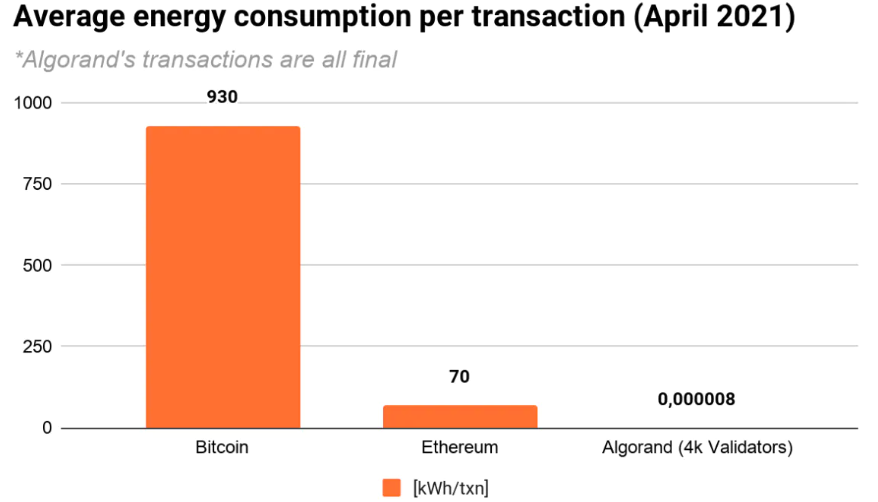
\includegraphics[scale=0.6]{images/schema_consumo.png}
\caption{Grafico dei consumi \cite{algorand_ambiente}}
\label{fig: graficoconsumi }
\end{figure}\\
Quindi, supponendo blocchi interi, mostriamo l'energia consumata dalle varie blockchain:
\begin{description}
    \item [Bitcoin] \begin{displaymath} E = 930 \: \frac{kWh}{txn} \end{displaymath}
    \item [Ethereum] \begin{displaymath} E = 70 \: \frac{kWh}{txn} \end{displaymath}
    \item [Algorand] \begin{displaymath} E = 0,000008 \: \frac{kWh}{txn} \end{displaymath}
\end{description}
Anche in questo caso, abbiamo evitato di appesantire il lettore con i calcoli. Per eventuali approfondimenti si rimanda all'articolo originale \cite{algorand_ambiente}.

\section{Sviluppi Futuri}

\subsection{Uso dei token}
Sicuramente un aspetto da non sottovalutare è quello relativo alla sicurezza dei sistemi mobili quando comunicano con lo smart contract. Nel progetto sviluppato nessuno può spacciarsi per un sistema centrale, infatti l'indirizzo pubblico di quest'ultimo viene memorizzato nella variabile globale \textit{Address Sistema Centrale} all'interno dello smart contract nella fase di opt-in di Intecs. Quando i metodi dello smart contract, costruiti appositamente per il sistema centrale, vengono chiamati (ci riferiamo a compare\_hash e validate\_snapshot), controllano che l'indirizzo mittente sia proprio uguale a \textit{Address Sistema Centrale}. Il problema risiede nel fatto che chiunque potrebbe fare opt-in allo smart contract e spacciarsi per un sistema mobile per richiamare il metodo \textit{insert\_local\_hash}. L'uso di token (gettoni) rappresenterebbe una soluzione al problema, in particolare l'uso di token che prendono il nome di \textit{asset token frozen} (token che si possono revocare), distribuiti dall'account Intecs ai vari account Algorand dei sistemi mobile come se fossero una sorta di "chiave" di accesso. Quando il sistema mobile invoca il metodo \textit{insert\_local\_hash} dello smart contract, mostrando il suo token, certifica che lui ha il permesso di fare quell'operazione. Detto in altri termini, dobbiamo far si che sia Intecs a poter dare l'ok ai sistemi mobile e questa implementazione la posso fare costruendo un account Intecs che crea token e ne dona uno ad ogni sistema mobile da usare come certificazione.

\section{Conclusioni}
Ritengo sia stato molto stimolante lavorare a questo progetto, visto che si tratta di una tecnologia in continua evoluzione che risulterà sempre più utilizzata nel futuro. Il progetto in sé, rappresenta un prototipo, per far capire quali possano essere le potenzialità della tecnologia blockchain e degli smart contract. Alcuni parti del progetto sono sicuramente migliorabili, ad esempio risulta macchinoso dover modificare manualmente i file di configurazione (JSON) ogni qualvolta si abbia la necessità di creare una nuova applicazione o di cambiare l'indirizzo Algorand pubblico del sistema centrale. Questa parte richiederebbe un'ulteriore approfondimento, che si potrebbe risolvere con l'utilizzo di un secondo smart contract gestito da Intecs SpA attraverso l'interfaccia a linea di comando intecs.py che memorizza l'indirizzo Algorand del sistema centrale e dell'application-id. Con tale sistema, ogni volta che viene modificato uno di questi valori, il programma intecs.py invia un segnale ai vari dispositivi per richiedere una nuova lettura delle variabili da questo smart contract e l'aggiornamento dei file di configurazione di tipo JSON.